\chapter{Реализация}
\label{chapter_implementation}

\section{Устройство инфраструктуры CPAchecker}
\label{sect_impl_cpachecker}

Фреймворк CPAchecker содержит в себе всю необходимую инфраструктуру для реализации различных подходов статической верификации.
Классический набор компонентов для верификации программного обеспечения является следующим: парсер, который преобразует исходный код программы во внутреннее представление, алгоритм, задающий правила работы с операторами CPA, сам набор CPA и автомат, который определяет нарушение спецификации.

В качестве парсера используется сторонний компонет Eclipse CDT Parser\footnote{https://eclipse.org/cdt}, который строит абстрактное синтаксическое дерево (англ. Abstract Syntax Tree, AST).
Далее, AST преобразуется в CFA, в этот момент выполняются такие преобразования, как добавление дуг ведущих внутрь функции и обратно в точку ее вызова, что необходимо для обеспечения межпроцедурности анализа.
Также, в этот момент собираются различные метаданные, которые затем могут быть использованы в процессе основного анализа: информация о переменных, циклах, зависимостях и т.п.

Исходный код программы, подаваемый на вход может быть разбит на несколько файлов, но, тем не менее, этот набор должен компилироваться.
Чтобы избежать сложных конструкций языка Си и упростить код, часто применяется инструмент CIL~\cite{CIL}, который, в том числе, может объединять несколько файлов в один.

Алгоритм задает правила работы с операторами CPA. Классический CPAAlgorithm был представлен в алгоритме~\ref{cpata_algorithm_ps}.
Кроме него могут использоваться и другие, например, BMCAlgorithm, PDRAlgorithm, реализующие BMC и PDR подходы к статической верификации соответственно.
Алгоритмы могут задавать комбинацию различных подходов, например, CEGARAlgorithm использует внутри вложенный алгоритм основного анализа, а при его завершении начинет итерацию уточнения.
RestartAlgorithm позволяет задавать последовательную комбинацию различных алгоритмов.

Любой алгоритм так или иначе требует определения CPA, с которыми он будет работать.
Используемый набор CPA определяет возможности проводимого анализа и его ограничения.
Почти во всех конфигурациях используются служебные CPA: LocationCPA и CallstackCPA. 
Различные примеры CPA были описаны ранее, и здесь нет смысла повторяться.

Для описания ошибочной ситуации используется автоматная модель. 
С помощью простого языка задается наблюдательный автомат, который совершает переходы в соответствии с графом потока управления одновременно с основным процессом анализа. 
Как только этот автомат доходит до некоторого терминального (ошибочного) состояния, считается, что найдена ошибка в программе.
Несмотря на то, что формат описания ошибки позволяет определять достаточно сложные условия, наиболее часто используется задание специальной функции, трактуемой, как ошибку.
В этом случае, автомат выглядит как
\begin{verbatim}
CONTROL AUTOMATON UNREACH

INITIAL STATE Init;

STATE USEFIRST Init :
  MATCH {__VERIFIER_error($?)}->ERROR("unreach-call");

END AUTOMATON
\end{verbatim}
Таким образом, вызов функции \_\_VERIFIER\_error, рассматривается, как ошибка. 
В процессе анализа автомат представляется в виде одного из CPA.

Такая спецификация используется для решения задачи достижимости, при которой проверяется, достижимо ли некоторое состояние программы, в данном случае, вызов функции \_\_VERIFIER\_error.
CPAchecker поддерживает и решение других задач, например, проверки корректного использования памяти или завершимости программы.
Такие задачи не описываются в виде спецификаций и могут быть решены только при специальной конфигурации Algorithm-CPA.

Реализация инструмента для поиска состояний гонки позволило добавить новый тип ошибки, который может быть найден инструментом CPAchecker.

\section{Общий вид инструмента для верификации многопоточных программ}
\label{sect_impl_lockator}

Как уже было описано, инструмент CPAchecker позволяет проверять программное обеспечение на соответствие различным типам спецификации.
Достижимость ошибочного состояния, корректная работа с памятью, завершаемость могут проверяться для многопоточных программ также, как и для последовательного случая.
Далее мы будет подробно рассматривать два основных варианта: проверка достижимости ошибочного состояния и поиск состояний гонки.

Основной набор CPA для каждого из этих вариантов остается неизменным: ThreadModularCPA (раздел~\ref{sect_impl_tm}), ARGCPA (раздел~\ref{sect_impl_arg}), CompositeCPA (раздел~\ref{sect_impl_composite}), LocationCPA (раздел~\ref{sect_impl_location}), CallstackCPA, LockCPA (раздел~\ref{sect_impl_lock}), ThreadCPA (раздел~\ref{sect_impl_thread}), PredicateCPA (раздел~\ref{sect_impl_predicate}).

\begin{figure}[ht] 
  \centering
  \includegraphics [scale=0.6] {CPATree}
  \caption{Вариант кобинации CPA}
  \label{img:CPATree}
\end{figure}
На рисунке~\ref{img:CPATree} показана типовая комбинация CPA для подхода с раздельным рассмотрением потоков.
CallstackCPA является служебным и отвечает за поддержку межпроцедурного анализа. Его реализация не изменилась по сравнению с классической версией, поэтому он не будет описан далее.
При поиске состояния гонки добавляется некоторый служебный UsageCPA (раздел~\ref{sect_impl_usage}), который позволяет упростить работу с доступами к сложным типам данных.
При решении некоторых практических задач не превый план может ставиться скорость анализа.
В этом случае может быть применена оптимизация BAM (раздел~\ref{sect_impl_bam}), которая позволяет существенно ускорить проведение анализа, но накладывает дополнительные ограничения на используемые CPA.
Далее реализация всех упомянутых CPA будет описана подробно.

Для определения состояния гонки необходимо было для каждой пары достигнутых состояний проверить наличие обращения к одинаковой разделяемой памяти.
Такой простой алгоритм был совершенно не эффективен для практического применения. Количество абстрактных состояний может превышать десятки миллионов.
Поэтому необходимы очень эффективные алгоритмы хранения и поиска пары состояний образующих состояние гонки. 
Такие оптимизации описаны в разделе~\ref{subsect_impl_storage}.

Процесс уточнения построенной абстракции может занимать достаточно много времени даже при решении задачи достижимости.
При поиске состояний гонки может быть необходимо уточнить абстракцию сразу для нескольких обнаруженных состояний гонки.
Уточнение абстракции последовательно становится очень неэффективным.
В разделе~\ref{sect_impl_refinement} описан процесс уточнения абстракции при поиске состояния гонки и применяемые оптимизации.

Важной задачей, на которую многие академические инструменты не обращают внимания, является понятное и наглядное представление результатов верификации.
Это особенно важно для описания ошибок, связанных с параллельным выполнением нескольких потоков, так как при этом не достаточно указать только строку или переменную, в которой возможно наличие ошибки.
Необходимо представить полную трассу выполнения потоков, выделив некоторые важные события, например, создание потоков, захват примитивов синхронизации и одновременные доступы к разделяемой памяти. В подразделе~\ref{sect_impl_visualization} будет описан формат выходных данных.

\section{Реализация ThreadModularCPA}
\label{sect_impl_tm}

Основное отличие реализации ThreadModularCPA от теоретического описания (раздел~\ref{sect_tm_cpa}) заключается в том, что в реализации применение переходов происходит до оператора $transfer$, а не после. 
Это приводит к тому, что все основные операторы -- $merge$, $stop$, $prec$ -- выполняются над проекциями, а не над примененными переходами.
Проекций значительно меньше, а очень многие проекции могут быть отброшены как покрытые, что позволяет значительно сократить количество элементов, к которым применяются эти операторы.
С точки зрения представленной теории такая операция не совсем корректна, так как композиция ($\epp$) проекции с любым другим переходом не даст ни одного конкретного перехода. 
В дальнейшем возможно определение расширенного оператора $\epp$, который позволит работать и с проекциями.
Однако, это не является темой данной работы, и поэтому данная оптимизация была представлена только в реализации.

Некоторые незначительные оптимизации связаны с сокращением количества проверок совместности состояния и проекции. 
Для этого определяются те состояния, к которым не имеет смысла применять проекции.
Такими состояниями могут быть либо инвариантные ко всем возможным проекциям, либо те, к которым в принципе невозможно применить ни одну проекцию.
Примером первого варианта могут быть состояния, в которых уже считается, что разделяемые данные принимают любые значения.
Примером второго варианта являются состояния, в которых известно, что активен только один поток.

\section{Реализация BAMCPA}
\label{sect_impl_bam}

\subsection{Краткое описание}
Сохранение результатов анализа абстрактных блоков (англ. Block Abstraction Memoization, BAM) является очень эффективной оптимизацией, которая основанна на кэшировании результатов. 
Абстрактными блоками, на границах которых производится кэширование результатов, могут быть как функции, так и тела циклов. 
При входе в абстрактный блок запоминается начальное состояние, а при выходе из него -- конечное.
И при следующем входе в этот абстрактный блок с тем же абстрактным состоянием, второй раз построение всего множество достижимых состояний не производится, а сразу выдается конечное состояние, взятое из кэша.

Для увеличения частоты попадания в кэш используются дополнительные операции $reduce$/$expand$, которые возвращают существенную для каждого внутреннего CPA часть абстрактного состояния.
Таким образом, можно избавиться от отличающихся, но несущественных деталей, которые мешали бы попаданию в кэш.
Обратная операция $expand$ возвращает утраченные детали в конце абстрактного блока на основе исходного состояния, в котором они присутствуют.

\begin{figure}[h]
\begin{minipage}[h]{0.3\textwidth}
\begin{verbatim}
  int g = 0;
   int f(int a) {
     return a + 1;
   }
   int main() {
     int l = 0;
     g = f(g);
     l = f(l);
     ...
  }
  
\end{verbatim}
\caption{Пример исходного кода}
\label{BAMCodeExample}
\end{minipage}
\hfill
\begin{minipage}{0.6\textwidth}
    \center{\includegraphics[scale=0.8]{BAMCPA-img.pdf}}
    \caption{Пример переходов BAMCPA}
    \label{img:BAMCPA}
\end{minipage}
\end{figure}

На рисунке~\ref{img:BAMCPA} показан пример работы BAMCPA.
При первом заходе в функцию f применяется операция $reduce$, которая определяет, что переменная $g$ не используется во внутреннем блоке (функции), и удаляет эту информацию из состояния. 
Таким образом, анализ функции производится с более абстракным начальным состоянием.
А при выходе из блока применяется обратная операция $expand$, которая возвращает прежнюю точность.
При втором заходе в функцию снова применяется операция $expand$, которая удаляет изменившееся значение переменной $g$, что позволяет получить точно такое же начальное состояние, а значит, попасть в кэш. 
Финальное состояние берется из кэша, к нему применяется операция $expand$, и анализ подолжается.

\subsection{Недостатки реализации}

BAM позволяет значительно сократить время работы инструмента при частых и однообразных вызовах функций.
Однако, такая оптимизация имеет и недостатки, которые существенным образом влияют на весь процесс анализа программы.
\begin{enumerate}
\item Множество достижимых состояний (reached set) становится неполным.
С учетом операции $reduce$ в нем могут отсутствать те состояния, которые были бы достижимы при анализе программы без оптимизации BAM.
Хотя операция $reduce$ и должна сохранить всю существенную для анализа информацию, отсутствующие детали могут не позволить использовать упрощенные состояния напрямую в некотором пост-анализе.
\item Множество достижимых состояний становится распределенным, то есть для каждого абстрактного блока создается своя копия множества достижимых состояний, в котором находятся все достижимые в данном блоке состояния, с учетом упрощения оператором $reduce$.
Такая копия необходима для удобства работы с кэшем.
\item Вычисление пути в графе достижимых состояний значительно усложняется из-за перечисленных выше пунктов. 
\item Все операции модификации множества достижимых состояний, в первую очередь при уточнении, становятся значительно сложнее, так как при любой модификации вложенного множества достижимых состояний необходимо проверить, как эта модификация затрагивает все остальные множества достижимых состояний.
\end{enumerate}

Эти сложности и недостатки были не очень существенными для классического анализа последовательной программы.
В случае подхода с раздельным рассмотрением потоков такие недостатки могут привести к некорректному результату.
Действительно, при вычислении возможных эффектов окружения на некоторое состояние, необходимо иметь доступ ко всему множеству достижимости, а в случае BAM это доступное множество ограничивается одним блоком.
Таким образом, применение BAM в текущем виде в подходе с раздельным рассмотрением потоков становится невозможным.
Одним из возможных направлений развития инструмента может стать реализация BAM в новой концепции, которая позволит сохранить монолитность множества достижимых состояний, что позволит расширить область ее применения на случай подхода с раздельным рассмотрением потоков.

В некотором частном случае применение BAM возможно. 
Это может произойти, если все вложенные CPA являются инвариантными к переходам в окружении, то есть применение проекций ни в каком случае не даст новых состояний.
В таком случае алгоритм анализа сводится к классическому, и ограничения BAM не смогут привести к некорректному результату.

\subsection{Особенности реализации при поиске состояния гонки}

Еще одна проблема, связанная с BAM, возникает при поиске состояний гонки. Она связана с  восстановлением пути, приводящего к ошибочному состоянию.
В исходном варианте оптимизации BAM состояние было только одно - ошибочное, соответственно, ошибка могла быть зафиксирована, если анализ обнаружил путь к этому конкретному состоянию.
В этот момент можно завершить построение абстракции и перейти к восстанавлению ошибочный пути и его уточнению.
При решении задачи достижимости найденная ошибка выдается как только она была найдена, и поэтому стек абстрактных блоков, приводящих к ошибке, восстанавливается единственным образом.
Если бы это было не так, то уже бы существовало как минимум два пути к ошибке, проходящих через различные абстрактные блоки.
Так как процесс анализа остается последовательным, то в этом случае данная ошибочное состояние было бы уже обнаружено при анализе первого абстрактного блока. 

При поиске состояний гонки приходится сначала строить все достижимые состояния, а затем искать те пары, которые образуют состояние гонки.
Это означает, что при восстановлении пути может возникнуть неопределенность, если одна из функций на стеке вызовов может быть вызвана из нескольких мест.
Такая неопределенность не может привести к некорректным результатам, однако она может повлиять на детерминированную работу инструмента, что значительно снижает удобство использования.

Для решения этой проблемы был сделан переработан механизм восстановления пути, для того чтобы восстановление возможных путей проводилась строго детерминированно.
При визуализации результатов нет необходимости показывать все возможные пути к некоторому доступу к памяти, однако в процессе уточнения необходимо проверить все варианты.
Подробнее про процесс уточнения результатов будет рассказано в соответствующем разделе.

\section{Реализация ARGCPA}
\label{sect_impl_arg}

ARGCPA отвечает за построение абстрактного графа достижимости (англ. Abstract Reachability Graph, ARG). 
Его состояния содержат в себе информацию о связях с другими состояниями.
Имеются следующие типы связей:
\begin{itemize}
\item parent-child. Связь соответствует оператору $transfer$, то есть дочерний элемент был получен из родительского путем применения оператора $transfer$ к последнему. 
У каждого дочернего элемента может быть множество родительских, например, из-за применения оператора $merge$, а также у каждого родительского может быть несколько дочерних.
\item covers-covered by. Связь соответствует оператору $stop$, то есть если оператор вернул true, то новый элемент считается покрытым старым. 
Следует отметить, что несмотря на теоретическую возможность покрытия множеством состояний, все реализации оператора $stop$ используют покрытие только одним состоянием.
Поэтому каждое абстрактное состояние может покрывать множество других, но быть поктыто только одним состоянием.
\item mergedInto.  Связь соответствует оператору $stop$ и означает, что один элемент был результатом вызова оператора $merge$ для другого состояния.
\end{itemize}

Данные типы состояний используются в разных целях: для визуализации, для построения контрпримера, для вычисления поддерева при уточнении.
Для подхода с раздельным рассмотрением потоков были добавлены две дополнительные связи:
\begin{itemize}
\item projectedTo-projectedFrom. Связь соответствует оператору $project$ и нужна, чтобы определить из какого исходного состояния была получена та или иная проекция.
\item appliedTo-appliedFrom. Связь соответствует оператору $apply$ и нужна, чтобы определить из каких состояний и проекций был получен тот или иной переход в окружении.
\end{itemize}

\section{Реализация LockCPA}
\label{sect_impl_lock}
Анализ примитивов синхнонизации соответствует описанному в теоретической части LockCPA (раздел~\ref{sect_lock_analysis}).
Теоретически описанный LockCPA имеет ряд допущений:
\begin{itemize}
\item захватываемый объект (блокировка) должен быть явно указан в операторе $acquire$/$release$;
\item никакие другие операторы, кроме $acquire$/$release$, не работают с примитивами синхронизации;
\item отсутствие рекурсивного захвата блокировки;
\end{itemize}

Однако, такие допущения не всегда выполняются при анализе реального кода. 

\subsection{Указатели на объекты блокировок}
В реальных же программах блокировки часто передаются в функцию захвата или освобождения по указателям.
При этом указатели могут храниться в полях различных структур.
Это значительно усложняет задачу определения реального объекта блокировки, с помощью которого производится синхронизация.
Во многих работах, которые посвящены вопросу применения инструментов статической верификации к реальному программному обеспечению, часто применяют анализ указателей для вычисления объектов, на которые могут указывать те указатели, которые используются при захвате блокировки.
Однако, как и всякий анализ указателей, такой подход имеет ряд недостатков, главными из которых являются его эффективность и точность.
Дело в том, что анализ указателей Андерсена (и его различные вариации) может применяться только если указатели должным образом инициализируются.
В случае же если инициализация указателя не была проведена, и этому указателю не была поставлена в соответствие некоторая память, такой анализ будет некорректным.
В нашем случае инициализация многих указателей может отсутствовать, так как не весь исходный код может доступен.

Все это приводит к тому, что определить точное соответствие указателей в общем случае становится невозможным.
Приходится делать некоторое разумное предположение о том, что захват блокировки и ее освобождение, скорее всего, будет производится одинаковым образом.
Например, если был использован указатель на объект при захвате, то он же будет использован и при освобождении.
А если при захвате использовался указатель на поле структуры, то и при освобождении будет передан указатель на поле с тем же именем и структуры того же типа.
Таким образом, становится возможно, в соответствии с теорией, по имени переменной, быть может указателю, явно идентифицировать тот объект, с которым производится работа.

\subsection{Неявные операции работы с примитивами синхронизации}
В пользовательских программах используется выделенный интерфейс для работы с примитивами синхронизации, который предоставляет операционная система.
В POSIX это функции pthread\_mutex\_lock/pthread\_mutex\_unlock. 
Однако, компоненты операционной системы внутри себя могут использовать различные примитивы синхронизации напрямую.
Например, проверять, включено ли планирование, которое также может выступать в роли особой (глобальной) блокировки.
При этом такая проверка может быть, как через специальный интерфейсный макрос/функции, например, $dispatchEnable()$, так и через явное обращение к переменной $dispatchLock == 0$\footnote{Пример кода является вымышленным, совпадение с какой-либо известной операционной системой является случайным}.
Кроме того, отключение планирование (захват блокировки) может также проводиться с помощью интерфейсного макроса/функции $dispatchLock()$ или напрямую $dispatchLock = 1$.
Хотя явное присваивание в служебные переменные без выделения интерфейсных макросов/функций является плохим стилем программирования, такой код иногда встречается на практике, и поэтому нуждается в поддержке.
Таким образом, реализация анализа примитивов синхронизации была расширена для обработки таких случаев, как присваивание в переменную и проверки ее значения.

\subsection{Рекурсивный захват блокировки}
Еще одной небольшой особенностью реализации является поддержка рекурсивного захвата блокировки. 
Некоторые блокировки допускают захват себя несколько раз в одном потоке.
В этом случае как только число вызовов функций освобождения будет равно числу ее захватов, она считается окончательно освобожденной.
В описанной теории такой случай не поддерживается, так как захваченные блокировки моделируются множеством.
В реализации достаточно просто поддержать рекурсивный захват, заменив множество на мультимножество.
Однако, в этом случае возможны ситуации с неконтролируемом ростом числа захваченных блокировок.
Это возможно как из-за ошибки в самом исходном коде, например, из-за захвата блокировки в цикле, так и из-за неточности самого анализа, например, рассмотрение недостижимого пути с отсутствующей парной операцией освобождения блокировки.
То есть, при реальном выполнении программы такой путь был бы невозможен, и для каждой операции захвата была бы соответствующая операция освобождения.
Но из-за неточности анализа анализа рассматриваются дополнительные пути, на которых отсутствует операция освобождения блокировки.
Классическим примером такой ситуации является захват и освобождение блокировки под одним и тем же условием. 
После выполнения такого участка кода при реальном выполнении ситуация, при которой эта блокировка останется захваченной, невозможна.
Однако, анализ может не определить, что условия являются тождественными, и будет рассматривать такой путь, при котором захват блокировки был произведен, а освобождения не было.
Такая ситуация чревата тем, что количество абстрактных состояний после анализа данного участка кода может удвоиться, то есть, после выхода из функции (или блока кода внутри функции) вместо единственного достижимого состояния без захваченных блокировок, будут рассматриваться состояния как без блокировок, так и с захваченной блокировкой.
И хотя такие шаблоны встречаются нечасто, все-таки обычно блокировки захватываются без сложных условий, необходимо иметь возможность давать анализу некоторые подсказки.

Такими подсказками стали аннотации функций.
Разработчик может добавить информацию о том, как именно следует обрабатывать конкретную функцию.
Поддерживаются следующие типы аннотаций:
\begin{itemize}
\item функция захватывает конкретную блокировку;
\item функция освобождает конкретную блокировку;
\item функция полностью сбрасывает конкретную блокировку, включая все рекурсивные захваты;
\item при выходе из функции все изменения блокировок сбрасываются, то есть, считается, что на выходе из функции захвачены те и только те блокировки, которые были захвачены на входе в функцию.
\end{itemize}

\subsection{Эффект блокировки}
Еще одно отличие от теории -- использование \textit{эффектов блокировок} -- было сделано больше для удобства, чем для эффективности.
С точки зрения теории оператор $transfer$ должен предоставить следующее (возможно, измененное) состояние.
В реализации этот оператор для каждой CFA дуги извлекает некоторое действие, которое она может совершить над состоянием. 
И затем, это действие применяется к состоянию. 
Выделения действия в отдельный интерфейс является не обязательной даже с точки зрения эффективности, так как даже на больших примерах время работы LockCPA находится в рамках статистической погрешности (меньше 0,1\% от общего времени работы).
Однако, выделение каждого изменения в отдельный класс упрощает структуру кода.
Так, имеются следующие варианты действия над состоянием:
\begin{itemize}
\item захват блокировки;
\item освобождение блокировки;
\item установка конкретного значения счетчика рекурсивного захвата блокировки;
\item восстановление заданного значения счетчика рекурсивного захвата для некоторой блокировки;
\item восстановление заданного значения счетчика рекурсивного захвата для всех блокировок;
\item проверка значения счетчика рекурсивного захвата для заданной блокировки;
\end{itemize}

\subsection{Оптимизация BAM}
\label{subsect_lock_bam}
Отдельно следует отметить оптимизации, сделанные в рамках подхода BAM, который описан в подразделе~\ref{sect_impl_bam}.
Как было описано, BAM позволяет кэшировать результаты, если некоторая часть состояния ($reduced$ $state$) совпадает с уже пройденным. 
При этом, чем менее уникальным состоянием будет $reduced$ $state$, тем эффективнее будет работать кэширование, то есть тем чаще будут возникать попадания в кеш.
С другой стороны, необходимо иметь возможность восстановить исходное состояние по $reduced$ $state$ в конце блока.
Очевидно, что если внутри блока не происходит никакого изменения состояния, то есть, внутри блока нет операций с примитивами синхронизации, то исходное состояние в конце блока равно исходному состоянию в начале блока, и в этом случае можно полностью удалять все захваченные блокировки. 
В этом случае кэш будет работать максимально эффективно с учетом работы других CPA.
При этом, конечно, остаются технические моменты, связанные с вычислением состояний гонки по завершению анализа.
Действительно, во множестве достижимых состояний сохраняются $reduced$ $state$, в которых могут отсутствовать те блокировки, которые используются для обеспечения взаимного исключения параллельной работы потоков.
В этом случае будет необходимо восстановить все утраченные блокировки после построения абстракции, о чем будет подробно рассказано в соответствующем разделе.

Одной из достаточно тривиальных оптимизаций для блоков, в которых производится работа с примитивами синхронизации, является удаление только тех блокировок, которые не затрагиваются этими операциями. 
Например, если известно, что в некотором блоке производится захват и/или освобождение блокировки $lock_1$, то из состояния можно удалить все остальные блокировки, а на выходе построить новое полное состояние, взяв изменение счетчика рекурсивных захватов $lock_1$ и добавив к нему значения счетчиков для других блокировок, взятые из исходного состояния. 
Такая оптимизация требует некоторого преданализа, результатом которого будет множество используемых блокировок для каждого блока.

Другой возможной оптимизацией является сокращение счетчика рекурсивных захватов.
Действительно, даже в случае, если внутри функции происходит захват/освобождение блокировки один раз, не имеет значения, сколько раз эта блокировка была захвачена до этого. 
Таким образом, при входе в функцию можно заменить значение счетчика рекурсивных захватов на единицу, а при выходе, соответственно, применить полученную разницу к исходному состоянию.
В случае применения этой оптимизации становится невозможным различить применение операции $release$ и $reset$, которая полностью сбрасывает счетчик рекурсивных захватов. 
Аналогичные проблемы вызывает операция установки конкретного значения счетчика рекурсивных захватов, хотя это исключительно редкая операция.
Более того, если в блоке используются более одной операции $acquire$/$release$ подряд, это становится аналогичным использованию уже описанных операторов.
Однако, все эти случаи встречаются достаточно редко, обычный сценарий использования - это захват одной блокировки в начале функции и освобождение ее в конце.
Отсюда следует, что указанная оптимизация может применяться только в тех блоках, в которых не используются такие запрещенные конструкции.

\subsection{Возможные вариации LockCPA}
\label{subsect_lock_merge}

Одним из возможных вариантов настройки LockCPA является реализация различных операторов $merge$ по аналогии с PredicateCPA.
$merge_{Sep}$ будет рассматривать все состояния по-отдельности, а $merge_{Join}$ -- объединять их в соответствии с решеткой, то есть, пересекать множества захваченных блокировок, строя т.н. множество $must$-блокировок.
Теоретически вариант $merge_{Join}$ должен уменьшить количество абстрактных состояний в случае, если возможны несколько путей, на которых захватываются различные блокировки, через одну точку программы.
При этом возможно снижение точности. 

Другим вариантом настройки LockCPA является использование уточнения.
Уже описанный вариант анализа отслеживает все указанные блокировки с самого начала. Однако, эти блокировки могут быть ненужными при построении абстракции, а значит, такая точность с самого начала может быть лишней.
Поэтому возможно применение метода CEGAR, с помощью которого будут определяться те блокировки, котороые являются необходимыми для исключения ложных сообщений об ошибке.
Основной вопрос заключается в том, будет ли выигрыш времени из-за построения неточной абстракции перекрыт проигрышем на некоторое количество дополнительных уточнений.
Ответы будут даны далее в разделе экспериментов.

\todo{Описание уточнения и merge}

\section{Реализация LocationCPA}
\label{sect_impl_location}
Анализ точек программы соответствует описанному в теоретической части LocationCPA: раздел~\ref{sect_location_analysis}
В целом, данный анализ не претерпел существенных изменений по сравнению с классической реализацией. 
Основной задачей было представить его работу в терминах переходов, то есть ввести понятие абстрактной дуги.
В классическом варианте анализа, LocationCPA оперирует дугами CFA, но для подхода с раздельным рассмотрением потоков пришлось дополнить это множество следующими специальными типами дуг:
\begin{itemize}
\item пустая дуга;
\item любая дуга;
\item отсутствие дуги.
\end{itemize}

Пустая дуга означает, что данный переход не меняет состояние LocationCPA и применяется в переходах в окружении.
Любая дуга означает, что данный переход может соответствовать любой CFA дуге и применяется в проекциях.
Технически, можно было бы обойтись одним вариантом для обозначения обоих случаев, но для удобства и отличия перехода в окружении от проекции были использованы различные служебные абстрактные дуги.
Отсутствие дуги требуется для обозначения ситуации, в которых отсутствует следующий переход.

\section{Реализация ThreadCPA}
\label{sect_impl_thread}
Анализ потоков соответствует описанному в теоретической части ThreadCPA: разделы~\ref{sect_thread_analysis},~\ref{sect_thread_analysis_env} и~\ref{sect_thread_analysis_ext}.
В зависимости от конфигурации запуска включается вариант ThreadCPA, основанный на той или иной версии теории.

\subsection{Ограничения реализации}

Важным отличием реализации данного анализа от теории является отсутствие жестко заданных идентификаторов потока. 
В теории идентификатором потока является точка входа в функцию потока. 
Соответственно, в этом случае становится невозможно поддерживать создание нескольких одинаковых потоков. 
Поэтому требуется некоторый явный идентификатор потока, который должен быть уникален.

В реальных языках используются различные интерфесы для создания потоков: POSIX, MPI, OpenMP и дл. 
Для системного программного обеспечения ближе оказывается интерфейс POSIX, в котором указывается некоторая переменная, в которой будет находится системный идентификатор потока, функция потока, ее аргумент, а также некоторые атрибуты. 
В этом случае идентификатором для анализа может выступать имя переменной, в которой должен находиться системный идетификатор потока.
Ограничением такого подхода является различные нестандартные ситуации, в которых происходит создание нового потока, с записью его идентификатора в переменную, в которой уже находится идентификатор другого исполняемого потока.
Такие ситуации не являются некорректными с точки зрения стандарта POSIX, но являются нетипичными для реального программного обеспечения.

Другим ограничением данного способа идентификации потоков является невозможность передачи идентификаторов через присваивания другим переменным. 
Так как для анализа потоков идентификатором потока является имя переменной, то присваивание системного идентификатора потока в другую переменную останется незамеченным.
Такие ограничения могут быть существенными для некоторого системного программного обеспечения, однако при решении конкретных прикладных задач автору не требовалась необходимость для расширения возможностей ThreadCPA.
Тем не менее, платформа CPAchecker позволяет переиспользовать различные анализы алиасов (синонимов) для решения этой задачи. 
Таким образом, данное ограничение хотя и может оказаться существенным для специфического программного обеспечения, само по себе не является критичным, и в случае необходимости может быть устранено с помощью существующих компонентов CPAchecker.

Еще одним ограничением эффективной релизации является неполная поддержка операций, типа $thread\_join$. 
В описанной теории данные операции не были описаны, хотя возможно расширение языка и формального описания ThreadCPA для поддержки таких случаев. 
В данной реализации предполагается, что ожидать завершения потока может только тот поток, который его создал.
В общем случае, это, конечно, может быть не так, однако, ситуация с передачей идентификатора дочернего потока от одного родительского потока другому для ожидания является необычной, и не встречалася в конкретных практических программах. 
Традиционная схема работы является следующей: один родительский поток создает несколько дочерних рабочих потоков (worker), раздает им задачи, а затем ожидает их завершения. 
Следует особенно подчеркнуть, что данное ограничение справедливо только для эффективной реализации, которая является инвариантной к эффектам окружения.
При использовании менее эффективной реализации, в которой используются переходы окружения для построения полного дерева потоков, нет никакой разницы, какой поток выполняет операцию $thread\_join$.

\subsection{Используемые оптимизации}
\label{sect_thread_create}
Одной из важных оптимизаций является обработка ситуации, при которой производится создание потока с уже существующим идентификатором. 
Как уже было описано в предыдущем подразделе, такие ситуации являются нестандартными при реальном выполнении программы, однако они могут возникать внутри анализа из-за его неточностей.
То есть, путь, в котором производится создание нескольких одинаковых потоков, является недостижимым при реальном выполнении.
В соответствии с подходом CEGAR можно было бы для каждого такого случая запустить процесс уточнения абстракции, а затем перестроить абстракцию заново с новым уровнем точности.
В целях повышения эффективности в процессе анализа такие ситуации не приводят к уточнению абстракции, а обрабатываются одним из двух следующих вариантов.

\begin{itemize}
\item После создания второго экземпляра (инстанса) потока, производится создание т.н. \textit{самопараллельного потока}, идея которого похожа на абстракцию счетчиков (англ. counter abstraction).
Это означает, что теряется информация о точном количестве созданных потоков, и считается, что все операторы этого потока могут быть выполнены параллельно друг с другом.
В этом случае становится бессмысленным дальнейшее создание потока, так как полученные состояния уже являются аппроксимацией сверху, и соответствуют любому количеству созданных потоков.
Для классических методов проверки моделей такая оптимизация приводит к значительной потере точности, но для подхода с раздельным рассмотрением потоков информация о возможных зависимостях между потоками уже потеряна.
Поэтому применение такой оптимизации при данном подходе не должна сильно снизить точность анализа.

\item Игнорирование создания второго и последующего потоков. 
Такой подход, в общем случае, может приводить к пропуску ошибок. 
Однако, в некоторых предположениях она позволяет получить корректные результаты.
Например, если имеется дополнительная информация, что поток всегда создается в единственном экземпляре.
Такая ситуация возникает, в ситуации, когда потоки являются искусственными, то есть не относятся к исходному коду программы, а лишь кодируют те части кода, которые могут выполняться параллельно.

\end{itemize}

\section{Реализация PredicateCPA}
\label{sect_impl_predicate}

\subsection{Обзор}
Анализ предикатов в целом соответствует описанному PredicateCPA в разделе~\ref{sect_predicate_analysis}.
Однако, его реализация содержит несколько особенностей, о которых не упоминалось в теоретическом описании, но о которых необходимо сказать в данном разделе, так как они оказывают серьезное влияние при реализации подхода с раздельным рассмотрением потоков.

Уточнение абстракции по контрпримерам (англ. Counterexample-guided abstraction refinement, CEGAR)~\cite{clarke:cegar},~\cite{CEGAR01} -- это подход для итеративного поиска точности анализа, который является достаточно строгим, чтобы доказать корректность программы, но достаточно грубы, чтобы быть эффективным. 
Анализ начинается обысно с пустой точности (пустого множества фактов, например, предикатов).
Построенная начальная абстракция программы является чрезмерной.
Если в этой абстракции было обнаружено некоторое ошибочное абстрактное состояние, то восстанавливается конкретный путь программы, который приводит к этому состоянию, и проверяется на достижимость.
Если такой путь является достижимым в исходной программе, то ошибка считается найденной, и анализ завершается.
В противном случае путь является недостижимым из-за неточной абстракции, и множество точности дополняется новыми фактами (уточняется) таким образом, чтобы исключить этот путь ошибки из абстракции.
Для предикатного анализа новые предикаты могут быть построены на основе вычисления интерполятора Крейга~\cite{CraigInterpol}. Эти шаги повторяются до тех пор, пока не будет найден конкретный путь ошибки или не будет доказана безопасность абстрактной модели (и, следовательно, программы).

Для улучшения про производительности применяется ленивая абстракция~\cite{LazyAbstraction}.
После шага уточнения алгоритма CEGAR абстракция перестраивается не полностью, а только те ее части, в которых необходимы новые предикаты.
Кроме того, новые предикаты не будут использоваться глобально для всех путей выполнения, а только в той части абстракции, для которых они актуальны.

Настраиваемое кодирование блоков (англ. Adjustable Block Encoding, ABE)~\cite{Beyer10} позволяет улучшить производительность предикатной абстракции за счет сокращения числа вычислений абстракции и числа итераций уточнения.
Новая абстракция вычисляется не для каждого нового абстрактного состояния, а в конце некоторого множества (блока) абстрактных состояний.
С ABE абстрактные состояния являются кортежами из абстрактной формулы и конкретной формулы пути.
Формула пути любого абстрактного состояния всегда представляет собой набор конкретных путей от входа блока до этого абстрактного состояния.
При создании нового абстрактного состояния вычисляется новая формула пути, которая является сильнейшим постусловием для предыдущей формулы пути и текущего ребра. Абстрактная формула копируется из предыдущего абстрактного состояния. 
Только в конце блока вычисляется новая абстрактная формула, которая является абстракцией конъюнкции старой абстрактной формулы и формулы пути.
В этот момент формула пути сбрасывается до $true$.
ABE не только сокращает количество вычислений абстракции, но также уменьшает количество проверок покрытия (которые выполняются только на концах блока) и размер ARG (из-за слияния абстрактных состояний).
Последнее сильно влияет на количество итераций уточнения, так как во время уточнения интерполянты вычисляются только для абстрактных состояний на концах блока, поскольку только для этих абстрактных состояний необходимы предикаты.

\subsection{Настраиваемое кодирование блоков}
\label{sect_predicate_abe}
Как уже было сказано, настраиваемое кодирование блоков (ABE) оказывает существенное влияние на эффективность проводимого анализа.
Однако, важной особенностью этой оптимизации является возможность проверки покрытия (оператор $stop$) только в конце блока. 
Для классического варианта реализации это позволяет уменьшить количество бесполезных проверок, так как количество состояний в конце блока не очень велико.
Однако, для подхода с раздельным рассмотрением потоков это может быть не так, так как к каждому состоянию внутри блока могут быть применены эффекты окружения для получения переходов в окружении. 
Если сразу же не отбросить их с помощью оператора $stop$, произойдет комбинаторный взрыв состояний.
А это значит, что классический вариант ABE становится невозможным, и приходится пересчитывать абстракцию после каждого состояния, чтобы получить возможность проверять покрытие состояний.

Таким образом, избежать частого пересчета абстракции, то есть получить некоторую вариацию ABE, станет возможно только если для текущего состояния удастся показать, что к нему невозможно применение эффектов окружения.
По общему виду состояния такое возможно определить, только если известно, что активен единственный поток.
Для этого необходим нетривиальный анализ потоков.
Такой вариант оптимизации позволяет исключить пересчет абстракции для самой начальной части пути, содержащей объявления переменных и типов.
Для больших программ эта часть может занимать серьезный объем, и даже такая простая оптимизация позволяет существенно повысить эффективность.

Следующим шагом является более интеллектуальная проверка, имеет ли смысл применять эффект окружения к текущему состоянию.
Эта идея восходит к давно известной редукции Липтона~\cite{Lipton} и заключается в том, что некоторые операции в потоке являются локальными, а значит, результат действия окружения перед этой операцией и после нее будет одинаковым.
Например, не имеет значения, как могут меняться глобальные переменные окружением, если текущий оператор потока записывает явное значение в локальную переменную.
А значит, к такому состоянию можно не применять эффекты окружения, отложив их до того момента, когда они станут релевантными операции.

С такой оптимизацией необходимо обращаться очень аккуратно, так как некорректное определение нерелевантных операций приведет к пропуску ошибки из-за того, что в нужный момент не был применен переход в окружении.
%Подробнее про реальные примеры?

\subsection{Представление эффектов окружения}
\label{sect_predicate_opt}
С точки зрения теории проекция перехода представляет собой пару из переименованных формул, соответствующих состоянию и действию. 
В реализации абстрактное состояние содержит абстрактную формулу и формулу пути.
Обе эти формулы записаны над переменными программы, однако формула пути использует SSA представление (англ. Single Static Assignment)~\cite{SSA}.
В этой форме присваивание в каждую переменную происходит лишь единожды.
На практике это достигается использованием SSA-индексов.
Соответственно, если применить действие другого потока в виде формулы пути, то используемые в этой формуле индексы старого потока станут некорректными в новом.

Были исследованы два варианта для представления эффектов окружения:
\begin{itemize}
\item Сохранять действие эффекта окружения в виде некоторого выражения, по которому каждый раз заново строить формулу.
Такой способ может быть реализован достаточно просто, однако, он снижает эффективность, так как каждый раз нужно заново построить формулу пути для этого выражения. 
Заметим, что никакое кэширование здесь не может быть использовано, так как необходимо получить формулу с уникальными индексами.
\item Сохранять действие эффекта окружения в виде формулы, но каждый раз вручную пересчитывать индексы переменных.
Такой способ позволяет проводить анализ более эффективно, так как не требуется перевычислять саму формулу каждый раз.
Однако, необходим аккуратный пересчет индексов. 
\end{itemize}

Таким образом, проекция перехода выглядит следующим образом: абстрактная формула, представляющая исходное состояние, и множество формул, которые описывают возможное действие.
Абстрактная формула будет использоваться для проверки совместности состояний. 
А множество атомарных формул представляют собой различные дизъюнкты, которые возникают при объединении нескольких эффектов.
Вместо такого множества можно было бы хранить одну большую формулу, но тогда это не позволило бы выбирать только релевантные дизъюнкты для каждого конкретного состояния.
Например, если эффект окружения кодирует изменение переменной, про которую нет информации в текущем состоянии, то нет смысла применять такой эффект, так как получившеесь состояние будет ниже по решетке, чем исходное и сразу же будет отброшено, как покрытое.
Таким образом, это множество позволяет применять только релевантные эффекты для каждого конкретного перехода.

%В теоретической части были описаны различные варианты оператора $merge$: $Join$, $Eq$ и $Sep$. 
Еще одной оптимизацией для увеличения скорости анализа является испльзование неизвестных значений при присваивании.
Во многих случаях становится неважным, как именно окружение может изменить разделяемые данные, и важно лишь то, что значение меняется.
А работа с точными значениями переменных требует затрат.
В таких случаях эффект окружения для каждого присваивания $x = 1$ может быть представлен в виде $x = *$, означающий, что значение переменной $x$ было изменено недетерминированным образом.
В качестве предельного случая может быть использован единственный эффект окружения $* = *$, который означает, что все разделяемые данные недетерминированно изменили свое значение.

Однако, получить результат, равносильный результату анализа с эффектом окружения $* = *$ можно значительно эффективнее.
Для этого необходимо построить такую модификацию предикатного анализа, которая была бы инвариантна к эффектам окружения.
В этом случае (см. раздел~\ref{sect_inv_analysis}) можно исключить ThreadModularCPA из конфигурации инструмента, что позволит существенно ускорить анализ.
При этом следует отметить, что в некоторых случаях результаты у этих двух вариаций анализа будут отличаться.
Это может произойти, если эффект окружения $* = *$ будет дополнен информацией от других CPA, например, ThreadCPA, который сумеет доказать, что данный эффект $* = *$ сбрасывает значения переменных только, если запущен некоторый поток.

\subsection{Уточнение абстракции}
\label{sect_predicate_refinement}
Процесс уточнения предикатной абстракции не описывался в теоретическом разделе, так как пока он принципиально не отличается от классического варианта уточнения, то есть не содержит серьезных изменений, специфичных для подхода с раздельным рассмотрением потоков.
Тем не менее, использование классического варианта уточнения является ограничением, которое не позволяет считать подход полным, так как некоторые ложные пути исполнения не могут быть удалены из абстракции в рамках классического варианта.

Как уже было сказано, при обнаружении ошибки запускается процедура уточнения CEGAR, первым шагом которой является восстанавление некоторого пути от начального состояния до ошибочного.  
Стоит отметить, что при использовании ABE такой путь может быть не один из-за того, что промежуточные абстрактные состояния могли быть объединены с помощью оператора $merge$. 
Восстановление пути происходит с учетом сохраненных связей ARG, что является технической задачей для классического анализа последовательной программы.
В случае многопоточной программы глобальный путь должен содержать действия каждого потока.
При этом, таких путей может быть снова некоторое множество.
Однако, в подходе с раздельным рассмотрением потоков невозможно восстановить возможные варианты чередования, так как эффекты окружения уже не имеют никакой информации о них.
Таким образом, с помощью классической процедуры восстановления пути становится возможным только получить локальный путь в отдельном потоке с точками воздействия эффектов окружения, то есть потенциальными переключениями на другие потоки. 
Это является серьезным ограничением, так как позволяет уточнять абстракцию в рамках только одного потока, и не позволяет ставить предикаты на эффекты окружения.
Поэтому одним из дальнейших направлений развития подхода является реализация возможности глобального уточнения, то есть восстановление пути с чередованиями в нескольких потоках.

Отдельным вопросом остается представление эффекта окружения в пути. 
Изначально путь представляет собой последовательность CFA дуг.
Соответственно, для некоторых эффектов окружения может не существовать таких дуг, которые бы полностью отражали его действие.
Более того, в случае, если эффект окружения включает в себя нетривиальные действия нескольких различных CPA, между ними возникнет конфликт, на основе какой информации подбирать подходящие дуги.
В данной реализации этот вопрос также не рассматривался, так как на практике всегда применялся анализ предикатов.
Напомним, что ни LockCPA, ни ThreadCPA, ни другие служебные CPA не используют никакого действия на другие потоки, а служат лишь для повышения точности оператора $compatible$.
Однако, при использовании ValueCPA и PredicateCPA параллельно друг с другом возможна ситуация, при которой эффект окружения будет построен на основе как перехода ValueCPA, так и перехода PredicateCPA.
Кроме того, возможны применения различных операторов $merge$, что приведет к полному рассогласованию связи перехода в окружении с исходными CFA дугами.
Таким образом, для представления полного пути с чередованиями будет необходимо разработать представление переходов, которое будет основано не на CFA дугах, а на более общих принципах, что также является одним из возможных направлений дальнейшего исследования.

Локальный путь в потоке тоже может содержать противоречия, и он может быть уточнен по классической схеме: для полученного пути строится логическая формула, она загружаются в специальный компонент \textit{решатель} (англ. solver), который возвращает новые предикаты.
Мы здесь не будем подробно касаться того, как именно могут извлекаться новые предикаты: на основе интерполянтов, инвариантов, слабейших предусловий или эвристик. 

Отметим лишь, что можно использовать различные схемы построения формул для пути для решателя.
\begin{itemize}
\item Классический вариант -- это извлечь уж построенную формулу пути из абстрактного состояния. 
Это должна быть именно формула пути, а не абстрактная формула, которая может быть менее точная.
\item Перестроить логическую формулу заново. Здесь открывается простор для различных оптимизаций, например, не учитывать разделяемые данные в формуле.
Такой вариант напоминает эффект окружения $* = *$, так как, по сути, игнорирование значений разделяемых переменных в формуле и означает, что они принимают любые значения.
Другим вариантом может быть перестроение логической формулы с учетом потенциальных эффектов окружения. 
Такой способ позволяет сократить время на перестроение абстракции, так как за одну итерацию уточнения позволяет получить расширенное множество новых предикатов.
\end{itemize}

\section{Реализация CompositeCPA}
\label{sect_impl_composite}

CompositeCPA объединяет все вложенные CPA в параллельную композицию.
Основное отличие реализации от теоретического описания заключается в том, что этот CPA позволяет работать как с теми CPA, которые реализуют подход с раздельным анализом потоков, так и с теми, кто его не релизует, считая, что абстрактные состояния этих CPA инвариантны к переходам в окружении. 
Таким образом, если доступна конкретная CFA дуга, переход осуществляется по ней, а если внутри перехода обнаруживается только абстрактная дуга, то переход по ней будет совершать сам анализ. 
В этом случае остальные CPA, которые не реализуют соответствующий интерфейс, не осуществляют переход, считая, что их состояние не изменяется.
Такой способ позволяет использовать различные существующие CPA, которые не реализуют соответствующий интерфейс.

Еще одной важной особенностью данного CPA является возможность реализовать оператор $merge$ специального вида. 
Дело в том, что внутренние операторы $merge$ не могут взаимодействовать друг с другом. 
Это значит, что каждый конкретный анализ должен самостоятельно решить, как он объединяет состояния.
Однако, на практике часто бывает полезно использовать объединение состояний одного CPA при некотором условии на состояния другого CPA.
Например, можно объединить все проекции для одного потока.
Это означает, что если два состояния ThreadCPA равны между собой, то в этом случае можно вызывать $merge$ у PredicateCPA.

Еще одним важным отличием от теоретического описания является использование более сложного оператора $\downarrow$ ($strengthen$). 
Дело в том, что вычисление необходимой CFA дуги для перехода может быть сделано более эффективно и без этого оператора.
Достаточно при выполнении оператора $transfer$ проверить, какой переход содержит LocationCPA внутри. 
В случае, если это CFA дуга, считается, что это переход в потоке, и все остальные CPA совершают переход по этой дуге.
В случае, если это некоторая заглушка, означающая, что переход пустой, это означает, что совершается переход в окружении, и все остальные CPA совершают переход в соответствии со своим имеющимся переходом.
Оператор $strengthen$ используется для отсеивания других бесмысленных переходов для повышения эффективности анализа.
\todo{Усиление}

\section{Реализация UsageCPA}
\label{sect_impl_usage}
Этот анализ используется только в конфигурации, которая применяется для поиска состояний гонки.
Исторически UsageCPA был сделан для того, чтобы он занимался эффективным хранением множества доступов к памяти.
Однако, в некоторый момент оказалось эффективнее перенести эту функциональность после основного алгоритма (см. раздел~\ref{sect_impl_races}).
Таким образом, в данный момент этот CPA реализует вспомогательные задачи по обработке специальных функций, анализ которых напрямую затрудняет работу инструменту.
Есть две основные группы таких функций:
\begin{itemize}
\item Функции работы со сложными структурам данных, например, списками.
\item Неопределенные функции, которые, тем не менее, имеют побочные эффекты.
\end{itemize}

Рассмотрим первую группу функций и возьмем для примера функцию, которая удаляет некоторый элемент из списка и возвращает его.
Внутри эта функция переставляет некоторым образом ссылки на элементы этого списка таким образом, чтобы он оставался консистентным.
Таких списков может быть несколько, которые устроены одинаковым образом, но используются по-разному, например, требуют различных механизмов синхронизации при работе с ними. 
Для анализа было бы удобнее считать, что при доступе к элементу этого списка, производится не только к этому элементу, а ко всему списку целиком. 
В таком случае появится возможность определить т.н. \textit{высокоуровневые гонки}, которые проявляются на сложных структурах памяти.
Таким образом, для каждой функции из первого множества, в конфигурации определяется пара доступов к памяти: один из них тот, к которому имеется непосредственный доступ, но каждый доступ к этой памяти после вызова указанной функции следует трактовать как второй доступ из этой пары.
Рассмотрим пример условной функции \textit{getLast()}, которая возвращает последний элемент списка: \textit{element = getLast(list)}.
Для такой функции может быть использована аннотация, которая определяет, что доступ к памяти $element$, которую возвращает эта функция, должен трактоваться как доступ ко всему списку $list$. 

Реальное программное обеспечение часто использует библиотеки, код которых недоступен для анализа.
Кроме того, такое программное обеспечение зачастую анализируется не целиком, а разбивается на некоторые модули, соответсвтвенно, код одного модуля недоступен при анализе другого.
Так или иначе, возникает некоторое множество неопределенных функций.
Часть из них можно было бы аннотировать, с какими разделяемыми данными производится работа внутри, что позволило бы получить более точные результаты.
Рассмотрим пример условной функции \textit{insertElement()}, которая вставляет элемент в список: \textit{insertElement(element, list)}.
Для такой функции может быть использована аннотация, которая определяет, что в этой функции производится доступ к памяти по указателю $list$, и этот доступ является записью, так как список может модифицироваться.


\section{Построение множества разделяемых данных}
\label{sect_shared_analysis}
При поиске состояний гонки может быть использован преданализ для построения множества разделяемых данных.
Это множество будет использовано на следующей стадии анализа, и при вычислении потенциального множества состояний гонки, для неразделяемых данных не будут выдаваться предупреждения.
На рисунке~\ref{img:method} представлена визуальная схема метода.

\begin{figure}[ht] 
  \centering
  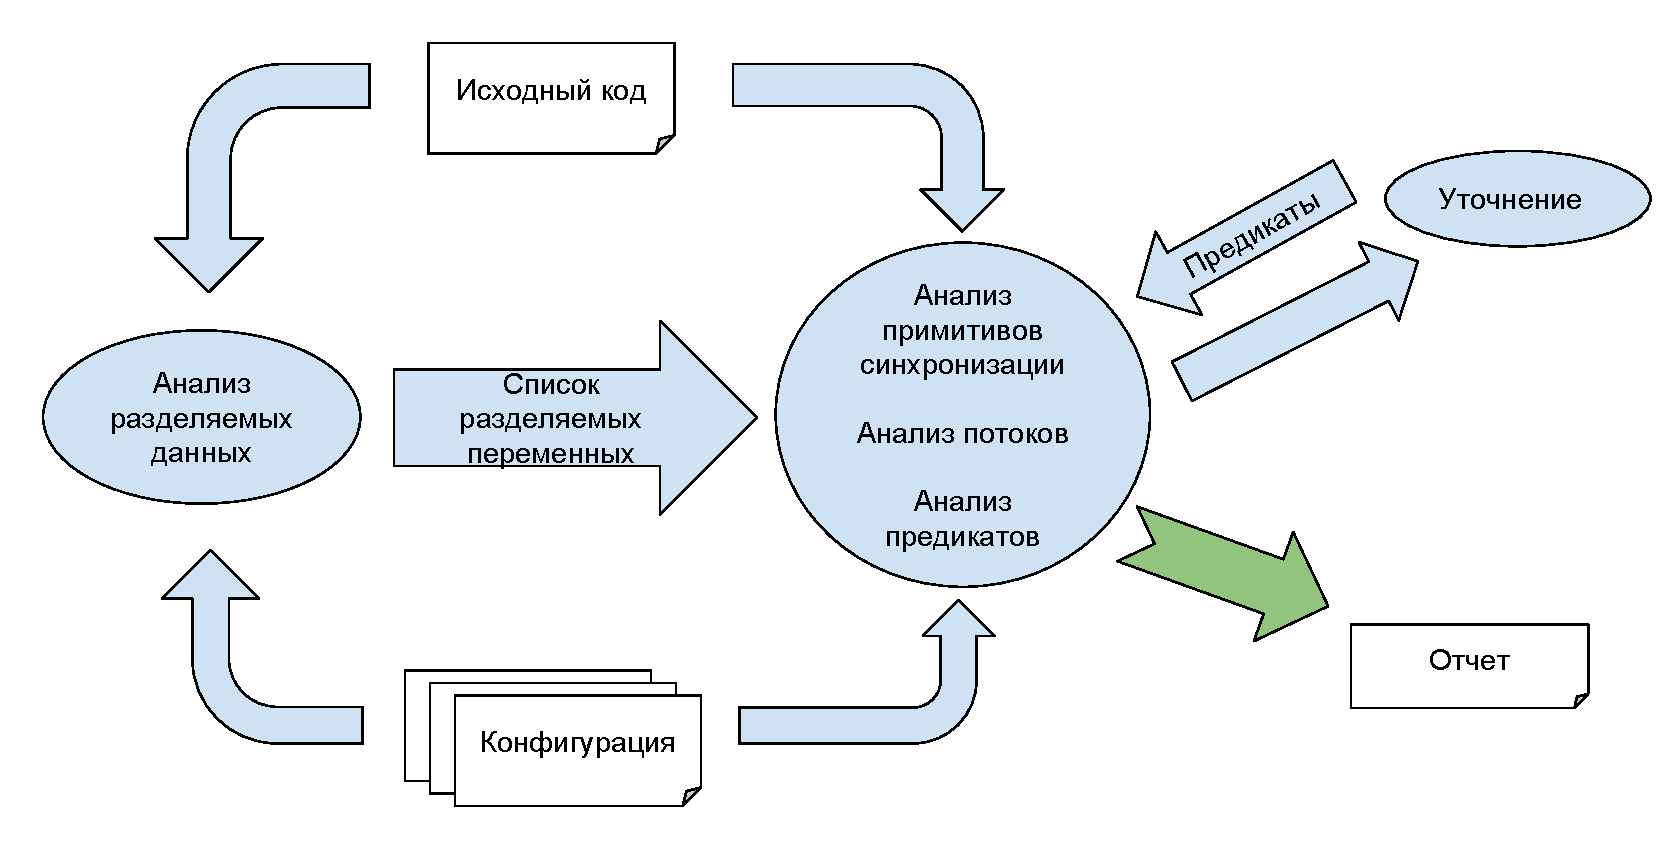
\includegraphics [scale=0.6] {MethodScheme}
  \caption{Общая схема метода}
  \label{img:method}
\end{figure}

Анализ разделяемых данных состоит из следующих CPA: BAMCPA, CompositeCPA, LocationCPA, CallstackCPA, ThreadCPA, LocalCPA.
То есть, все CPA, кроме LocalCPA используются в основном анализе и уже были описаны ранее, поэтому в данном разделе будет представлено только описание LocalCPA, которая и реализует всю функциональность для определения разделяемых данных.

Данный CPA является инвариантным к переходам в окружении, так как вся возможная информация об указателях консервативно объединяется.
То есть, некоторая переменная становится разделяемой в некоторой точке программы, то считается, что это переменная стала разделяемой для всех путей выполнения проргаммы, в том числе и для всех потоков.
Поэтому описание LocalCPA будет произведено в терминах классического CPA, то есть без описания абстрактных переходов и проекций, которые являются лишними для такого простого варианта анализа.

Будем использовать множество статусов $S = \{shared, unknown, unshared\}$, которые обозначают, что соответсвующий указатель является разделяемым, неизвестным и неразделяемым.
Абстрактным доменом LocalCPA является множество всех возможных отображений из переменных $X$ в их статусы $S$: $\forall e \in E, e=\{(x, s) \mid x \in X, s \in S\}$.
Соответственно, в состоянии хранится информация о текущем отображении.

Опишем формальные правила преобразования состояний оператором $transfer$.
Отдельно следует отметить, что рассматривается статус именно тех данных, на которые указывает переменная, если она соответствующего типа.
Нет необходимости следить за глобальными переменными, так как они в любой момент являются разделяемыми и за локальными переменными, так как к ним нельзя получить доступ из другой функции, а значит, и из другого потока.
Таким образом, имеет смысл сохранять информацию о статусе только тех переменных, которые являются указателями.
Однако для сбора такой информации требуется знания о локальности самих переменных.
Будем обозначать $local$ и $global$ информацию о локальности самих переменных.
Не нужно путать их со статусом той памяти, на которую указывает переменная.

Рассмотрим некоторое состояние $e$ и некоторый переход по дуге $g$, который соответствует некоторому оператору программы. 
Опишем, как может измениться $e'$.

\begin{enumerate}
\item Объявление локального указателя указателя добавляет информацию, что память, на которую он указывает, неразделяемая: $e' = e \cup \{a \to unshared\}$.

\item Правила обработки присваивания $a = b$:
\begin{itemize}

\item Для переменных, не являющихся указателями, а также для присваиваний переменным некоторых констант, состояние не меняется: $e' = e$.

\item При присваивании локальному указателю другого, статус последнего присваивается первому.
$e' = e \cup \{a \to e(b)\}$.

\item При присваивании глобальному указателю разделяемыми становятся данные, на которые указывал присваиваемый указатель.
$e' = e \cup \{b \to shared\}$.
Данное присваивание следует понимать так, что если в старом состоянии $e$ было какое-либо значение для $e(b)$ оно заменяется на $shared$.
Следует напомнить, что в целях оптимизации данные про глобальный указатель $a$ не добавляются в состояние.

\item После взятия адреса у локальной переменной $a = \&b$ $а$ указывает на неразделяемые данные.
$e' = e \cup \{a \to unshared\}$.

\item После взятия адреса у глобальной переменной $a = \&b$ $а$ указывает на разделяемые данные.
$e' = e \cup \{a \to shared\}$
\end{itemize}

\item Условия сами по себе не меняют состояние анализа $e' = e$.

\item Обработка вызовов функций. 
\begin{itemize}
\item При вызове функции статус указателя, передающегося, как параметр в функцию, присваивается этому параметру.
Кроме этих присваиваний в функцию не передается ничего, так как глобальные указатели не сохраняются.
То есть вся информация о статусе переменных вызывающей функции становится недоступна в вызываемой функции.
При вызове функции $f(a)$, $e' = \{p \to e(a)\}$, где $p$ -- это параметр функции.

\item При передаче в качестве параметра адреса глобальной переменной статус параметра становится shared.
При вызове функции $f(\&a)$, $e' = \{p \to shared\}$, где $p$ -- это параметр функции.

\item При передаче в качестве параметра адреса локальной переменной статус параметра становится unshared.
При вызове функции $f(\&a)$, $e' = \{p \to unshared\}$, где $p$ -- это параметр функции.

\item При вызове функции, возвращающей значение, сначала обрабатывается вызов функции в соответствии с правилами, описанными выше, а затем, согласно п. 2, обрабатывается присваивание возвращенного значения в переменную.

\end{itemize}

\item Во время возврата из функции состояние возвращается к тому, что было при ее вызове. 
При наличии добавляется информация о статусе возвращаемого значения.

\item Пустые операции не меняют состояние.
\end{enumerate}

Отдельно следует отметить вычисление статуса для памяти, на которую указывает поле структуры.
\begin{itemize}
\item Если соответствующая информация сохранена в состоянии напрямую для $a \rightarrow f$, то результатом будет этот статус.
\item Если соответствующая информация для $a \rightarrow f$ неизвестна, но сохранен статус для объемлющей структуры $a$, то результатом будет этот статус для структуры $a$.
\end{itemize}

Оператор $merge$ объединяет информацию от нескольких путей анализа, примером может являться две ветви условного оператора.
Состояние $e' = merge(e_1, e_2, \pi)$ является таким отображением, для которого выполнено следующее условие: $\forall x \in X, e'(x) = max(e_1(x), e_2(x))$, где $shared$ > $unknown$ > $unshared$.
Таким образом, оператор merge реализует консервативность анализа: если на каком-то пути переменная может стать разделяемой, а на другом нет, она будет считаться разделяемой в дальнейшем анализе.

\section{Вычисление состояний гонки}
\label{sect_impl_races}

\subsection{Обзор}
\label{subsect_impl_race_overview}
Вычисление состояний гонки происходит после завершения основного алгоритма анализа, то есть после полного построения множества достижимых состояний.
Основной задачей такого постанализа является определение и сохранение информации о доступах к данным. 
Доступ к памяти представляется некоторым идентификатором, структура которого будет представлена в подразделе~\ref{subsect_impl_identifiers}.
Для каждого оператора программы определяются те доступы к памяти, которые могут быть затронуты при его выполнении, определяется тип доступа и некоторая вспомогательная информация, например, номер строки исходного кода.
Подробнее структура сохраняемой информации будет представлена в подразделе~\ref{subsect_impl_storage}.

Поддерживаются следующие типы операторов:
\begin{itemize}
\item Присваивание. Для левой части присваивания формируется идентификатор (множество идентификаторов) и добаляется тип доступа на запись, для правило части присваивания формируется идентификатор (множество идентификаторов) и добавляется тип доступа на чтение.
\item Условие. Формируется идентификатор (множество идентификаторов) с типом доступа на чтение.
\item Вызов функции. Для каждого аргумента формируется идентификатор (множество идентификаторов) с типом доступа на чтение.
\item Возврат из функции. Для возвращаемого значения формируется идентификатор (множество идентификаторов) с типом доступа на чтение. В случае, если возвращаемое значение присваивается в некоторую переменную, для этой переменной формируется идентификатор (множество идентификаторов) с типом доступа на запись.
\end{itemize}
Определения переменной без присваивания, пустые (служебные) операторы не считаются доступами к памяти.

Информация о доступе перед сохранением проходит ряд тривиальных фильтров, которые позволяют избежать хранения бесполезной информации о тех доступах к данным, которые не могут участвовать в состоянии гонки.

\begin{itemize}
\item Запись в локальные переменные. Так как локальные переменные доступны только одному потоку, то изменение их значения не может быть одновременным.
\item Запись в неразделяемую память. Например, сразу после выделения новой памяти она еще недоступна другим потокам, и ее можно изменять без использования механизмов синхронизации.
\item Запись в служебные переменные, например, те, которые используются в модели окружения для обеспечения корректной последовательности вызовов. 
\end{itemize}

После построения множества доступов к памяти, для каждого идентификатора необходимо определить, существует ли пара доступов, которая образует гонку.
Каждая пара доступов проверяется на совместность, то есть на возможность одновременного выполнения
Для этого используется понятие совместности переходов. Совместность означает, что два частичных абстрактных состояния могут быть частью одного глобального состояния.
Или, другими словами, один переход может быть применен, как переход в окружении, к другому переходу и наоборот, откуда следует, что эти два перехода могут быть выполнены параллельно.
Таким образом, предложенный подход является обобщением подхода Lockset~\cite{eraser}, который определяет состояние гонки, как два доступа к некоторой памяти с непересекающимся множеством блокировок.
Одним из ограничений подхода Lockset является отсутствие поддержки других типов синхронизации.
В расширении подхода для этого используется оператор compatible. 
Так как проверка совместности использует различные типы анализа, включая анализ примитивов синхронизации, анализ предикатов и другие, такой способ является более точным, чем алгоритм Lockset.
Если обнаружена пара совместных доступов к данным, которые образуют состояние гонки, проверка остальных доступов для данного идентификатора прекращается.
Таким образом, для каждого идентификатора может быть выдано не более одного предупреждения о потенциальном состоянии гонки.

\subsection{Идентификаторы доступа к памяти}
\label{subsect_impl_identifiers}

Обычно под состоянием гонки подразумевается ситуация, при которой имеет место одновременный доступ к некоторой памяти из разных потоков, причем один из доступов должен быть записью.
Два основных вопроса, которые возникают при статическом поиске гонок: как определить, что доступ производится к одной и той же памяти, и как определить одновременность доступов.
Дальше будут подробно представлены эти две особенности в предлагаемом подходе.

При описании формальной модели программы использовался простой императивный язык программирования, который поддерживает разделяемые данные, представленные только глобальными переменными.
В реальном программном обеспечении используется большое количество операций с указателями, структурами и более сложными типами данных.
Как уже отмечалось в обзоре, многие точные инструменты статической верификации, в частости инструменты, реализующие методы ограничиваемой проверки моделей, вообще не распространяют свои подходы на программы с указателями, ограничиваясь только глобальными переменными.
В других инструментах, про которых уже говорилось в при обзоре, применяется анализ синонимов (англ. alias) Андерсена.
В этом случае собираются так называемые may-алиасы для каждой переменной, то есть множество областей памяти (адресов), на которые может указывать данный указатель.

Для нашей задачи поиска состояний гонки в системном программном коде не подходит первый способ, так как основная работа с памятью производится по указателям.
Поиск алиасов для каждого из нескольких тысяч указателей является слишком трудоемкой задачей.
В итоге необходимо использовать некоторую разумную эвристику, которая позволит определить одну и ту же область памяти. 
В предалагаемом подходе для этого используется модель памяти BnB, которая разделяет всю память на непересекающиеся множества регионов.
Каждый регион относится к одному типу данных или полю структуры, в случае если у него не брался адрес.
Такая модель памяти имеет ряд ограничений. В первую очередь, она не полностью поддерживает адресную арифметику и кастирование, что накладывает некоторые дополнительные условия на применимость подхода.
Кроме того, она может приводить к ложным предупреждениям об ошибках, в случае если два указателя одного типа никогда не указывают на одну и ту же память.

Основой предложенной эвристики стало наблюдение, что обычно указателями на один тип данных в системном программном обеспечении работают похожим образом.
Так, например, в один и тот же указатель обычно записывают похожие данные, которые защищаются одинаковым способом.
В этом случае не обязательно отслеживать с помощью точного анализа алиасов, на какую память конкретно может указывать некоторый указатель.
И если к нему обращаются различными способами, например, с использованием примитивов синхронизации и без них, то это уже является достаточно подозрительным местом.
При этом встречаются случаи, в которых такая эвристика дает ложные срабатывания, например, если имеются два доступа к различным объектам того же типа.

Отдельно имеет смысл подчеркнуть, что для простых типов регионы соответствуют типам.
А для полей структур, у которых не брался адрес регион будет отдельный от того типа, к которому принадлежит это поле структуры.
Такая оптимизация позволяет сократить число ложных предупреждений об ошибках из-за неравенства двух объектов.
Действительно, если у поля структуры никогда не брался адрес, то доступ к этому полу возможен только снова с использованием имени этого поля.
При этом не имеет значение, как происходит доступ к родительской структуре.
Исключением может стать доступ к памяти с использованием адресной арифметики.
% Однако, практика показывает, что в реальном системном программном обеспечении адресная арифметика обычно используется для вычисления некоторого


\subsection{Оптимизации хранения данных}
\label{subsect_impl_storage}

После построения абстракции для каждого найденного перехода вычисляются все доступы к данным на нем.
Эти доступы к данным сохраняются в глобальном контейнере, который затем будет обеспечивать эффективную работу с ними, в том числе поиск.

\subsubsection{Описание доступа к данным}

Для каждого доступа к данным формируется специальная структура данных, содержащая информацию об этом доступе. 
Будем использовать обозначение $usage$ для этой структуры данных.
$usage = (usage\_core, states)$, где $usage\_core = (node, access, state, path, id)$. Здесь 

\begin{itemize}
\item $node \in Loc$ -- узел CFA, которому соответствует данный доступ;
\item $access \in \{READ, WRITE\}$ -- тип доступа;
\item $state \in E$ -- соответствующее абстрактное состояние из анализа, которое используется для восстановления пути;
\item $states \in 2^E$ -- множество состояний различных анализов, которые должны учитываться при определении состояния гонки;
\item $path$ -- найденный истинный путь к данному использованию;
\item $id$ -- идентификатор переменной, описанный в подразделе~\ref{subsect_impl_identifiers}.
\end{itemize}

Состояние $state$ является полным состоянием, которое включает в себя все абстрактные состояния вложенных CPA. 
А множество $states$ включает в себя абстрактные состояния только тех CPA, которые будут использоваться для проверки совместности.
Состояния LockCPA, содержащие множество захваченных блокировок, используются для определения потенциальных состояний гонки, поэтому состояния этого анализа присутствуют во множестве $states$. 
В текущей конфигурации кроме состояний LockCPA используются состояния ThreadCPA. 

$path$ содержит путь, ведущий из начального состояния программы к данному доступу.
Путь состоит из набора CFA дуг, а не из абстрактных состояний. Это необходимо для эффективного расходования памяти.
Дело в том, что из-за специфики сборщика мусора Java, вся память, на которую имеются ссылки, не может быть освобождена.
Это приводит к тому, что любое сохраненное абстрактное состояние приводит к тому, что в памяти хранится полный граф достижимости.
Сам по себе он занимает достаточно много места, а несколько его экземпляров (с учетом уточнения) могут привести к исчерпанию ресурсов.
Поэтому приходится хранить небольшие объекты -- CFA дуги, которые, тем не менее, позволят в случае необходимости воспроизвести путь.

Множество всех $usage$ будем обозначать, как $UsageSet$. 

\subsubsection{Определение доступов к данным}

Технически определение возможных доступов к данным является несложной операцией.
Для каждого перехода из множества достижимых состояний нужно повторить следующий набор шагов:

\begin{enumerate}
\item определить множество доступов к данным на этом переходе;
\item проверить, имеет ли смысл хранить полученный доступ;
\item для каждого релевантного доступа построить соответствующий $usage$;
\item дополнить построенный $usage$ утраченной из-за BAMCPA информацией, чтобы получить полное описание;
\item сохранить полное описание $usage$ для последующего поиска состояния гонки.
\end{enumerate}

Основная проблема в этом алгоритме заключается в восстановлении полного описания.
Как уже было описано ранее, для повышения эффективности BAM может удалять некоторую информацию из состояния с помощью операции $reduce$.
Для LockCPA эта операция может удалять блокировки, если они не используются в текущем блоке.
Тем не менее, эти блокировки являются существенными для поиска состояний гонки.
В данный момент только LockCPA модифицирует свое состояние, но в дальнейшем возможно появятся и другие CPA.
Поэтому для каждого найденного доступа необходимо восстановить всю утерянную информацию.

Именно поэтому был выделен отдельный элемент $usage\_core$. 
Для абстрактного перехода исходный $usage$ строится только один раз, а затем он может быть несколько раз модифицирован, в зависимости от того, сколько возможных путей, ведущих через различные абстрактные блоки было обнаружено в процессе анализа.
Чтобы не копировать $usage$ целиком, все неизменяемые элементы выделены в отдельный блок, который не копируется при восстановлении.

\subsubsection{Эффективный поиск состояний гонки}

Одной из задач глобального контейнера является обеспечение быстрого поиска состояний гонки среди всех добавленных доступов.
Если бы все найденные $usage$ хранились как обыкновенное множество, то перебор всех возможных пар занимал бы слишком большое время.
Однако, условие совместности двух доступов, которое и необходимо проверить для окончательного вердикта, зависит только от информации в $states$.
Еще одно требование -- это хотя бы один доступ на запись.
Таким образом, первой идеей является отказ от лишней информации при поиске состояний гонки.
Поэтому на верхнем уровне контейнера для каждого идентификатора переменной содержится множество $point$.
$point$ -- это срез информации, содержащейся в $usage$, которая может повлиять на наличие состояние гонки: $states$ и $access$.
Каждому $point$ может соответствовать несколько реальных $usage$. 
И в этом случае пространство поиска существенно сокращается.
Таким образом, если будет найдено состояние гонки в терминах $point$, любое из соответствующих им $usage$ также будут образовывать состояние гонки.

Следующим шагом является исключение из поиска заведомо бессмысленных случаев.
Если имеется $point$ с меньшим количеством блокировок, то его имеет смысл рассматривать в первую очередь.
Например, $point_1$ содержит внутри $states$ состояние LockCPA, в котором находится только одна блокировка $lock_1$.
А $point_2$ содержит две блокировки $lock_1$ и $lock_2$.
Какое бы парный $point_3$ мы не взяли, имеет смысл рассматривать с ним только $point_1$, так как если существует состояние гонки с $point_2$, будет иметь место и состояние гонки с $point_1$.
При этом возможны ситуации, в которых состояние гонки будет иметь место только в паре с $point_1$.

Конечно, такая оптимизация требует полного покрытия всех состояний из $states$.
То есть, если состояния LockCPA покрываются, а состояния ThreadCPA несравнимы, то в этом случае отбросить соответствующий $point$ будет некорректным.
Формально говоря, необходимо упорядочить $states$ и рассматривать только верхние элементы.
При этом, конечно, таких элементов может быть несколько, так как используется лишь частичный порядок.

Пока мы не интересовались истинностью найденных состояний гонки.
То есть, все описанные оптимизации основывались на том, что все скрытые $usage$ и $point$ равноценны оставшимся с точки зрения достижимости.
Однако, не все найденные доступы возможны при реальном выполнении с учетом дополнительной информации $states$.
Например, может оказаться, что доступ к данной переменной производится только под блокировками, так как соответствующий путь, ведущий к доступу к этой переменной без блокировок, является невыполнимым.
В этом случае необходимо перейти к следующему пути, следующему $usage$ или следующему $point$.
Подробнее сам процесс уточнения и различные его оптимизации будут представлены в подразделе~\ref{sect_impl_refinement}.

В случае, если путь является достижимым, становится бессмысленно проверять другие пути, ведущие к данному $usage$.
Более того, становится ненужным проверять и другие $usage$, соответствующие тому же $point$.
Поэтому полученный достижимый путь сохраняется в поле $path$ у соответствующего $usage$, a соответствующий ему $point$ тоже помечается, как достижимый.
Это необходимо для того, чтобы не проверять каждую итерацию уточнения те пути, для которых уже была доказана их достижимость.
Действительно, на одной из итераций уточнения может возникнуть ситуация, при которой для одного доступа будет найден достижимый путь, а все остальные доступы, которые могли образовать с ним состояние гонки, будут отброшены, как недостижимые.
После этого необходимо заново перестроить уточненную абстракцию, чтобы проверить, появятся ли эти доступы снова.
Если доступы будут обнаружены, то к ним уже будут вести другие пути, которые снова необходимо проверить на достижимость.
При этом проверять достижимость первый путь уже будет не нужно, так как он должен существовать и в более точной абстракции.
Если для некоторой переменной были найдены два истинных пути, которые образуют состояние гонки, значит, больше нет необходимости собирать информацию для этой переменной.
Она помечается специальным образом и больше не участвует в уточнении.

\subsubsection{Пример представления данных}
\label{subsect_impl_example}

Рассмотрим такой фрагмент исходного кода.

\begin{verbatim}
int global;
...
int dummy_function(){
  int local;
  ...
  global = 1;
  mutex_lock(&mutex);
  local = global;
  mutex_unlock(&mutex);
  ...
  mutex_lock(&mutex);
  local = local + global;
  mutex_unlock(&mutex);
}
\end{verbatim}

Часть контейнера для этого фрагмента программы представлена на рисунке~\ref{img:globalcontainer}. 

\begin{figure}[ht] 
  \centering
  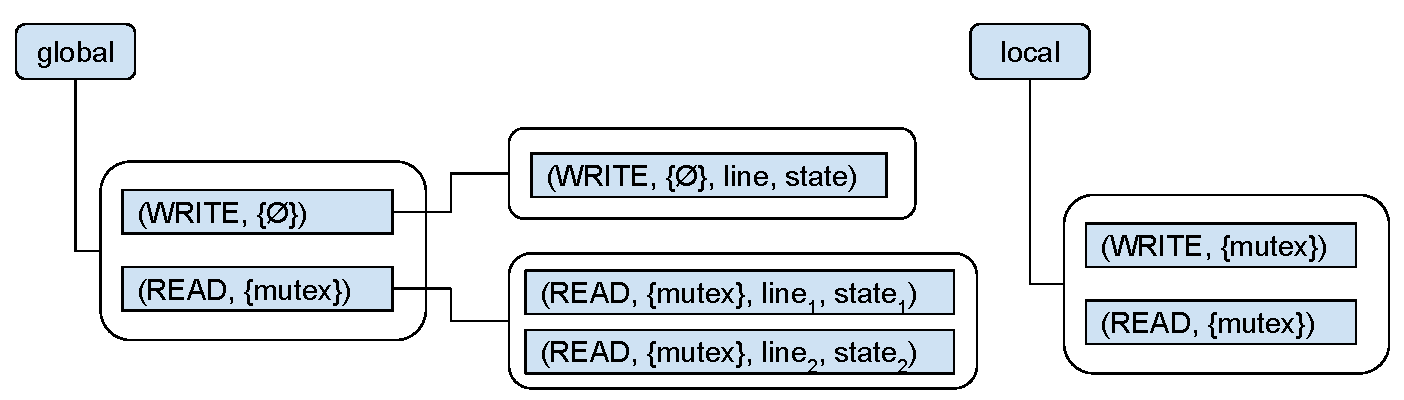
\includegraphics [scale=0.7] {GlobalContainer}
  \caption{Пример}
  \label{img:globalcontainer}
\end{figure}

Переменной $global$ соответствуют две точки использования: запись без использования примитивов синхронизации и чтение при захваченной mutex-блокировке. 
Причем второй точке использования соответствуют два реальных доступа, расположенных в разных строках исходного кода.

\section{Реализация уточнения при поиске состояний гонки}
\label{sect_impl_refinement}

\subsection{Общее устройство}
Уточнение абстракции по контрпримерам используется для того, чтобы исключить недостижимые пути из абстракции.
В классическом варианте работы CPAchecker CEGAR используется при решении задачи достижимости.
В случае, если найдено ошибочное состояние, начинается процесс уточнения: строится контрпример и проверяется, возможен ли такой сценарий выполнения в исходной программе.
Еесли такой путь является недостижимым из-за неточности абстракции, она уточняется таким образом, чтобы исключить такой путь из абстракции. 

При поиске состояний гонки дело усложняется тем, что ошибкой является не одно состояние, а пара. При этом каждый из путей сам по себе не является ошибкой.
Кроме того, обычно требуется обнаружить не первое состояние гонки в программе, а все потенциальные состояния гонки. 
Таким образом, возможны две вариации процедуры уточнения абстракции.

\begin{enumerate}
\item Уточнение производится в процессе анализа. При обнаружении пары состояний, составляющих состояние гонки, оба пути проверяются на достижимость.
Если найденная ошибка подтверждается, она отмечается, как подтвержденная, и анализ продолжается.
Этот вариант уточнения очень похож на классический вариант: при обнаружении ошибки абстракция уточняется до тех пор, пока ошибка либо не подтвердится, либо не опровергнется.
Такой подход обладает существенным недостатком: для корректного завершения анализа, требуется построить очень точную абстракцию. 
В случае, если анализируемый код содержит сотни тысяч строк кода, построение точной абстракции требует колоссального времени. 
Более эффективно в этом случае гибко задавать ограничения на ресурсы, чтобы иметь возможность завершить анализ в любой момент, хотя это и повлечет за собой некоторое снижение точности. 

\item Уточнение всех путей производится в тот момент, когда абстракция полностью построена.
Все обнаруженные состояния гонки проверяются на истинность, и, в случае необходимости, абстракция перестраивается. 
Существенным недостатком этого подхода является большой объем лишней работы в том случае, если неточность абстракции затрагивает множество состояний гонки.
Тогда проверка каждой из них будет давать один и тот же результат.
Однако, возможно применение некоторых оптимизаций, которые позволяют сократить время на такую бесполезную работу. 

\end{enumerate}

%Нужно отметить, что оба варианта уточнения способны исключать из абстракции только локально-недостижимые пути.
%Пути, в которых неправильно моделируется взаимодействие потоков, не могут быть исключены из абстракции.

Для того, чтобы обеспечить гибкую настройку, процесс уточнения был разделен на функциональные блоки.
Каждый такой блок определяется тем, что он принимает себе на вход от предыдущего блока, и тем, что он выдает на выходе следующему.
Результатом работы каждого из абстрактных блоков является вердикт $true$, означающий, что то, что передается на вход этому блоку, содержит состояния гонки, и вердикт $false$, означающий, что состояние гонки обнаружить не удалось.
В последнем случае может быть выдана некоторая информация (precision), которая позволит более точно вычислить абстракцию на следующей итерации анализа.
В редких случаях возможен вердикт $unknown$, означающий, что однозначный ответ не может быть получен. 
В большинстве случаев такой вариант реализуется при некорректной работе сторонних компонентов, таких как решателей (англ. solver).

На рисунке~\ref{img:RefinementSceme} представлен возможный вариант последовательности функциональных блоков при уточнении. 

\begin{figure}[ht] 
  \centering
  \includegraphics [scale=0.5] {RefinementSceme-img}
  \caption{Последовательность функциональных блоков при уточнении}
  \label{img:RefinementSceme}
\end{figure}

Цепочка блоков уточнения состоит из двух частей. Первая часть - служебная, которая используется для подготовки путей к уточнению и обработке полученной от других блоков информации. Эта часть содержит:

\begin{enumerate}

\item IdentifierIterator. Блок, принимающий на вход ReachedSet и последовательно перебирающий все возможные переменные, к которым был доступ.
Соответственно, следующий за ним блок обязан принимать на вход идентификатор переменной.
В случае, если хотя бы для одной переменной был получен вердикт $false$, это означает, что уточнение прошло успешно, и необходимо перестроить абстракцию.
Если же для всех новых переменных вердикт был $true$ или $unknown$, это означает, что абстракция построена с достаточным уровнем точности, и все найденные состояния гонки являются истинными с точки зрения анализа.

Каждый вердикт $false$ сопровождается некоторой информацией о том, как следует уточнить абстракцию.
Этот уровень точности сохраняется для каждой переменной отдельно, но при построении абстракции учитывается уровень точности, полученный для каждой из переменных.
Однако, в случае если для  какой-либо переменной будет доказано, что она участвует в истинном состоянии гонки, то соответствующий этой переменной уровень точности сбрасывается.
Это помогает не перестраивать слишком точную абстракцию тогда, когда это уже не нужно.

\item PointIterator. Блок, принимающий на вход идентификатор переменной и перебирающий все возможные пары $point$, которые образуют состояние гонки.
Каждая пара $point$ проверяется следующим блоком. Если для некоторой пары $point$ будет получен вердикт $true$, это означает, что ни один следующий блок не смог найти противоречия, а значит, полученное состояние гонки истинное, и в предыдущий блок возвращается результат $true$. 

\item UsageIterator. Блок, принимающий на вход пару $point$ и перебирающий все возможные пары $usage$, соответствующие этой паре $point$.
Каждая пара $usage$ проверяется следующим блоком. Если для некоторой пары $usage$ будет получен вердикт $true$, это означает, что ни один следующий блок не смог найти противоречия, а значит, полученное состояние гонки истинное и в предыдущий блок возвращается результат $true$. 

\item PathIterator. Блок, принимающий на вход пару $usage$ и перебирающий все возможные пары путей в абстракции, соответствующие этой паре $usage$.
Необходимо пояснить, почему в абстракции возможно несколько путей из начального состояния к тому состоянию, которое соответствует данному $usage$.
Дело в том, что из-за применении оптимизации BAM (подраздел~\ref{sect_impl_bam}), тело функции будет проанализировано один раз, несмотря на то, что вызовов этой функции может быть несколько.
В таких случаях для каждого вызова функции возможно несколько точек ее вызова.
Если для некоторой пары путей будет получен вердикт $true$, это означает, что ни один следующий блок не смог найти противоречия, а значит, полученное состояние гонки истинное и в предыдущий блок возвращается результат $true$. 

\end{enumerate}

Далее идет вторая часть цепочки, которая занимается непосредственно проверкой корректности двух путей.
Поэтому каждый из этих блоков принимает на вход и передает в следующий блок пару путей.
Если текущий блок считает, что данная пара путей невозможна, в предыдущий блок возвращается результат $false$.
Блоки уточнения из этой части не являются обязательными, поэтому допустима любая их комбинация.

\begin{enumerate}

\item PredicateRefiner. Основной инструмент для удаления из абстракции локально-недостижимых путей. 
Использует внутри себя классический алгоритм уточнения для предикатного анализа, но дополнительно применяется некоторый набор оптимизаций для того, чтобы сократить время работы.
Например, при переборе всех возможных пар путей может часто возникать проверка отдельного пути на локальную-достижимость. 
Чтобы избежать лишних проверок, сохраняется результат каждого уточнения для пути, а также тот уровень точности, который нужен для исключения данного пути из абстракции.
Таким образом, если возникнет необходимость в уточнении этого же пути, не важно на этой же итерации уточнения или на любой из последующих, выдет использован сохраненный результат. 

Возможны различные варианты реализации

\item LockRefiner. Анализ примитивов синхронизации (LockCPA) может отслеживать все состояния блокировки без применения уточнения.
Причем обычно каждый захват блокировки делается для того, чтобы исключить некоторое потенциальное состояние гонки.
Однако, для больших программных систем не обязательно учитывать все блокировки каждый раз при пересчете абстракции.
Если доказано, что данная переменная не может участвовать в состоянии гонки, можно исключить из рассмотрения те захваты блокировки, которыми она защищалась, что позволит сократить время на следующий пересчет абстракции.

%\item Фильтр. Фильтром называется такой блок, который, выдавая результат FALSE, не предоставляет уровень точности для того, чтобы исключить полученный путь (пару путей) из абстракции. А это значит, что такая же пара путей будет получена и для следующей абстракции.
%Такой фильтр, тем не менее, полезен тем, что при переборе всех подходящих путей может быть найдена такая пара, которая будет истинна.
%Возможны различные варианты фильтров, например, такой, который отсеивает доступы к переменным, происходящим из специальных функций. 

\end{enumerate}

% Последний блок в цепи является специальной заглушкой, которая всегда возвращает значение TRUE.
\subsection{Оптимизации}

Основной проблемой при уточнении множества путей в одной абстракции является неизбежное повторение получаемых противоречий.
Например, если в абстракции не учитывается некоторое значение переменной в условном операторе, в этом случае все проходящие пути через этот условный оператор будут содержать это противоречие и, следовательно, будут недостижимы по одной и той же причине.
Было бы эффективнее избегать уточнения тех путей, которые проходят через точки программы, для которых были установлены новые факты (precision) ранее.
В качестве точек программы можно использовать:

\begin{itemize}
\item узлы CFA;
\item состояния ARG.
\end{itemize}

В первом случае критерий становится более слабым, что позволяет отложить уточнения большего числа путей.
Стоит отдельно заметить, что отложенные пути не выбрасываются из абстракции.
Таким образом, даже в случае неверно принятого решения из-за слабости критерия, они не будут полностью выброшены, а появятся снова на следующей итерации уточнения.

Однако, восстановление пути тоже занимает достаточно большое количество времени.
Поэтому полностью строить путь для того, чтобы оценить, через какие точки программы он проходит, становится неэффективно.
Приходится в процессе восстановления пути проверять, не проходит ли уже промежуточный отрезок пути через какие-нибудь повторяющиеся точки программы.

\section{Печать и визуализация} \label{sect_impl_visualization}

\subsection{Общая схема визуализации}
Визуализация найденных состояний гонок является важным моментом для практического применения инструмента.
Выдаваемой информации должно быть достаточно для того, чтобы разработчик смог понять, какие именно действия в программе могут привести к состоянию гонки.
Таким образом, основными требованиями к визуализации являются:

\begin{enumerate}

\item Отображение всех операторов, которые встречаются на пути к каждому из доступов, образующих состояние гонки

\item Отображение и визуальное выделение двух доступов, образующих состояние гонки

\item Отображение и визуальное выделение всех операций с примитивами синхронизации

\item Отображение справочной информации о состоянии гонки: множество захваченных примитивов синхронизации, тип и имя разделяемой переменной

\end{enumerate}

Основой формата вывода найденных состояний гонки является graphml формат, описанный в~\cite{SVCOMP15},~\cite{Witness}.
Этот формат предполагает преставление пути к ошибке в виде графа, который описывает путь от начального состояния программы до состояния, соответствующего ошибке.
Ребра графа соответствуют дугам графа потока управления.

Путь в графе имеет линейную структуру, хотя формат позволяет описывать различные ветвления, например, циклы, которые удобнее визуализировать, не разворачивая все выполненные итерации.
Так как разработанный инструмент реализует метод с раздельным рассмотрением потоков, то мы не может однозначно указать порядок выполнения инструкций (чередование потоков).
Лишь те места, где имеется применения эффектов окружения, могут интерпретироваться как возможные переключения потоков.
Поэтому в визуализируемом пути выполнения все инструкции каждого потока идут последовательно друг за другом.
Главный поток выполняется до точки, в которой происходит разделение путей, ведущих к двум доступам к памяти.
Обычно, это происходит при создании некоторого потока.
После этого продолжается первый путь, который приводит к первому доступу к памяти.
Далее отображаются операторы второго пути, начинающиеся с той точки разветвления.
Таким образом для пользователя будет выведено сначала трасса, ведущая к первому доступу, а затем, трасса ко второму доступу.

Пример визуализированной трассы представлен на рисунке~\ref{img:error_trace}.

\begin{figure}[ht] 
  \centering
  \includegraphics [scale=0.5] {ErrorTraceExample}
  \caption{Пример визуализированного предупреждения}
  \label{img:error_trace}
\end{figure}

Визуализация graphml представления производится инструментом Klever.

\subsection{Оптимизации при визуализации}

\subsubsection{Визуализация только истинных ошибок}

Как уже было отмечено в соответствующем разделе, реализация процесса уточнения после построения абстракции позволяет завершить анализ в любой момент времени и выдать все найденные предупреждения.
При этом полученный результат будет аппроксимацией сверху потенциально возможного результата при бесконечном количестве времени.
То есть все потенциальные ошибки будут найдены при первом же построении абстракции, а все остальное время будет тратиться на то, чтобы исключить ложные с точки зрения достижимости пути.

Таким образом, для удобства анализа экспертом можно выдавать только те ошибки, которые были подтверждены при уточнении.
При этом, конечно, будет возможен пропуск реальной ошибки, если она не успела подтвердиться, однако такой режим и не подразумевает доказательство корректности программы.

\subsubsection{Фильтрация одинаковых путей}

Зачастую работа в критической секции под блокировками содержит несколько операторов.
Например, даже простая операция занесения элемента в список требует модификации поля добавляемого элемента и поля элемента в списке.
В случае некорректной синхронизации, скорее всего, будут получены предупреждения для обоих доступов к памяти.
Однако, причина ошибки у них одна и та же, поэтому нет смысла анализировать эти предупреждения несколько раз.

Для этого используется следующая эвристика. Для каждого доступа к данным формируется идентификатор: фунция и множество состояний $states$ из $usage$.
Если для некоторой пары доступов, образующей состояние гонки, соответствующая им пара идентификаторов уже была выдана ранее для некоторого другого предупреждения, это означает, что такое состояние гонки является повторяющимся и может быть отфильтровано.

%\newpage
%============================================================================================================================

\clearpage